\chapter{Workspace characterisation and its consequences}
\label{ch:workspace}

This chapter is separated from \cref{ch:results} because it is not a single
measurement but a chain of them, and because its consequences determined the
shape of the task set. It reports a negative finding together with a
quantified and buildable mechanical fix; the finding alone would be a
complaint rather than a contribution.

\section{Continuous reachability from the home pose}

Reachability was measured as a swept extent rather than as pointwise
feasibility, because teleoperation requires the arm to travel to a pose from
where it already is, without a branch change. Twenty-six directions were swept
in \SI{1}{\centi\metre} steps from the home configuration, each step seeded
from the previous solution exactly as the follower does.

Repeating the sweep ten times gave identical quartiles: the inter-quartile
range was \SI{0.000}{\metre} in every direction for both arms. The measurement
repeats. What did \emph{not} repeat in earlier runs was the summary statistic:
isotropy taken as the minimum over directions of a single sweep is dominated
by rare early terminations and varied by a factor of two between runs. On
medians it is stable, at \num{0.16} for the left arm and \num{0.10} for the
right (\cref{fig:reach}).

\begin{figure}[htbp]
  \centering
  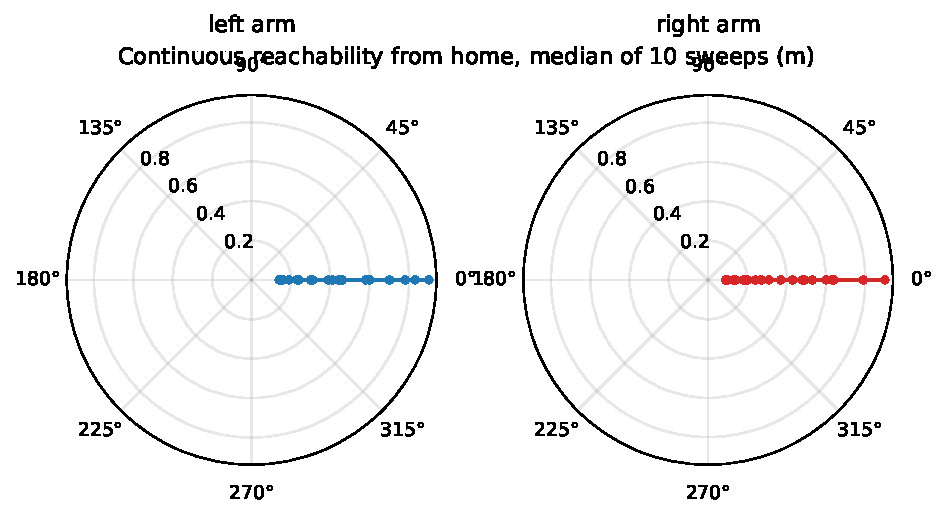
\includegraphics[width=\textwidth]{figures/reachability_polar.pdf}
  \caption[Continuous reachability from home]{Continuous reachability from the
  home pose, median of ten sweeps, projected onto the horizontal plane. The
  envelope is markedly anisotropic: the median reach is
  \SIrange{0.34}{0.40}{\metre} but the worst direction is
  \SI{0.14}{\metre} on the left arm and \SI{0.09}{\metre} on the right.}
  \label{fig:reach}
\end{figure}

The early terminations were traced to the measuring tool rather than to the
robot. A sweep is a chain of up to ninety solver calls and any single failure
ends that direction; the follower does not suffer this because it re-seeds the
redundant joint and retries. Giving the sweep the same retry reduced early
terminations from nine to zero on the left arm and three to zero on the right,
while the medians barely moved. That the medians were already right is what
establishes the outliers as chain compounding rather than geometry.


\begin{figure}[htbp]
  \centering
  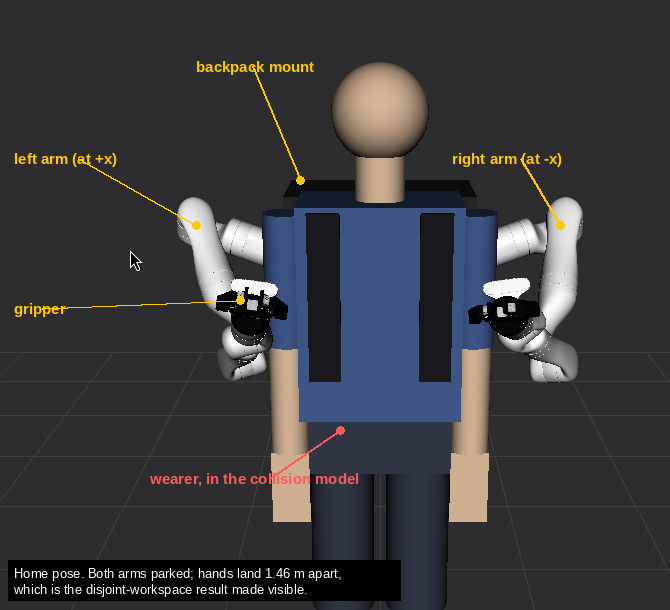
\includegraphics[width=0.72\linewidth]{figures/rviz/home_pose_labelled.png}
  \caption[The mounted configuration at the home pose]{The simulated platform
  at the home joint angles, captured from the running system rather than
  drawn. Both arms are parked over the shoulders and both hands finish on the
  same side of the body, \SI{1.46}{\metre} apart. That asymmetry is not a
  rendering artefact and not a mount error: it follows from the home joint
  angles, which are ground truth because the simulation-to-hardware bridge
  replays them onto the real arm. It is the disjoint-workspace result of this
  chapter made visible.}
  \label{fig:rviz-home}
\end{figure}

\section{The two arms share no reachable workspace}

Over a grid of sixty-three cells spanning the frontal working volume, with the
arms verified at the home pose, \textbf{no cell was reachable by both arms}.
The result survives the two obvious objections, as \cref{tab:overlap} shows:
freeing the wrist yaw raises each arm's individual reach from sixteen and eighteen
cells to twenty-one and still yields no shared cell, and repeating the test
with more redundancy retries changes nothing.

\begin{table}[htbp]
  \centering
  \caption[Both-arm overlap under three test conditions]{Both-arm overlap over
  the 63-cell frontal grid, arms verified at home. The null result survives
  both wrist freedom and additional inverse-kinematics retries.}
  \label{tab:overlap}
  \begin{tabular}{lccc}
    \toprule
    Test condition & Both & Left & Right \\
    \midrule
    Fixed orientation, 3 retries & \textbf{0/63} & 16 & 18 \\
    Fixed orientation, 6 retries, 3 repeats & \textbf{0/63} & 17 & 18 \\
    Yaw free, 6 retries & \textbf{0/63} & 21 & 21 \\
    \bottomrule
  \end{tabular}
\end{table}

A fine sweep in \SI{0.05}{\metre} steps across the plane on which the arms
would have to meet locates the boundary precisely: the right arm reaches
$x \le \SI{-0.10}{\metre}$, the left reaches $x \ge \SI{0.15}{\metre}$, and
there is a \SI{0.25}{\metre} dead band between them in which neither arm can
place its end effector (\cref{fig:disjoint}).

\begin{figure}[htbp]
  \centering
  
\includegraphics[width=0.9\textwidth]{figures/workspace_disjoint.pdf}
  \caption[The measured dead band]{The two reachable sets do not meet. Measured
  at $y=\SI{0.35}{\metre}$, $z=\SI{1.10}{\metre}$ with yaw free and three
  repeats per point.}
  \label{fig:disjoint}
\end{figure}

\subsection{What this does and does not establish}

It establishes that, within $x \in [-0.6, 0.6]$, $y \in [0, 0.4]$,
$z \in [0.90, 1.30]$~\si{\metre}, with the as-built mount and the legacy home
joint angles, the two reachable sets do not intersect.

It does \emph{not} establish behaviour outside that volume, nor does it
generalise to other mounts. The correct claim is that the arms share no
workspace \emph{as mounted and as parked}, and the remedy is mechanical.

\section{The fix is buildable}

A parametric sweep over candidate mount placements shows the null result is
not intrinsic. Moving the mounts inboard, forward and down, with additional
forward tilt, raises the number of shared cells from three to
\textbf{twenty-two} on the purely kinematic measure, within a buildable
\SI{0.20}{\metre} mount separation (\cref{fig:mount}).

\begin{figure}[htbp]
  \centering
  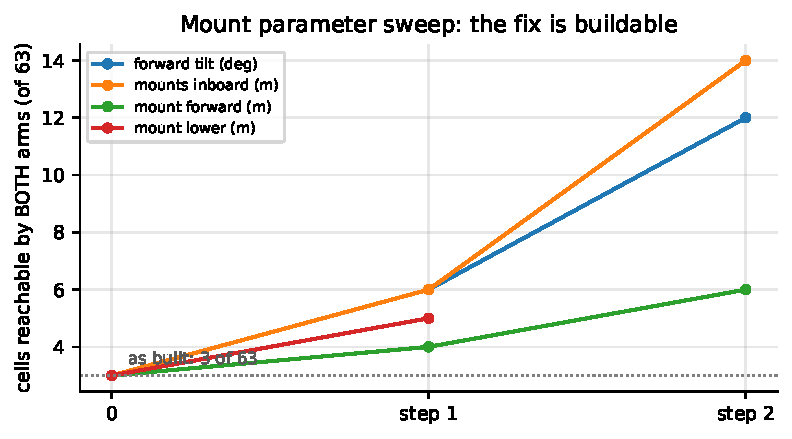
\includegraphics[width=0.85\textwidth]{figures/mount_sweep.pdf}
  \caption[Mount parameter sweep]{Single-parameter sweeps from the as-built
  mount. Forward tilt and inboard translation both help substantially; splaying
  the mounts outward \emph{hurts}. The sweep is purely kinematic, moving the
  arms' bases without moving the wearer, so these are upper bounds and any
  candidate requires a clearance check before adoption.}
  \label{fig:mount}
\end{figure}

The sweep was recorded and deliberately not applied, because changing the
mount invalidates the home pose, the workspace anchor and every clearance
figure reported in \cref{ch:results}.

\section{One boundary, two independent constraints}

Two further measurements, taken for different reasons, land on the same
lateral boundary and together make the case that the inboard band is
unusable.

The first is wearer clearance. Every scenario in the chest-height band passes
inverse kinematics with collision checking enabled, and the planner reports
the poses valid, yet the arms pass within \SIrange{48}{67}{\milli\metre} of
the wearer's torso, inside the \SI{120}{\milli\metre} margin the real-robot
configuration enforces. The reconciliation is that the two tests ask different
questions: the planner's check is binary contact, whereas the floor is a
margin, and a pose can satisfy one while being refused by the other. Sweeping
the lateral half-span shows clearance rising monotonically and crossing the
floor at \SI{0.25}{\metre}.

The second is grasp feasibility. A top-down grasp requires the wrist to adopt
an orientation with its approach axis vertical. Sweeping the same lateral
coordinate gives a sharp cliff: zero of nine grasp candidates are solvable at
$|x| = \SI{0.25}{\metre}$ and nine of nine at $|x| = \SI{0.30}{\metre}$. The
failure persists with collision checking disabled, so it is kinematic
infeasibility of the wrist orientation rather than obstruction.

\begin{figure}[htbp]
  \centering
  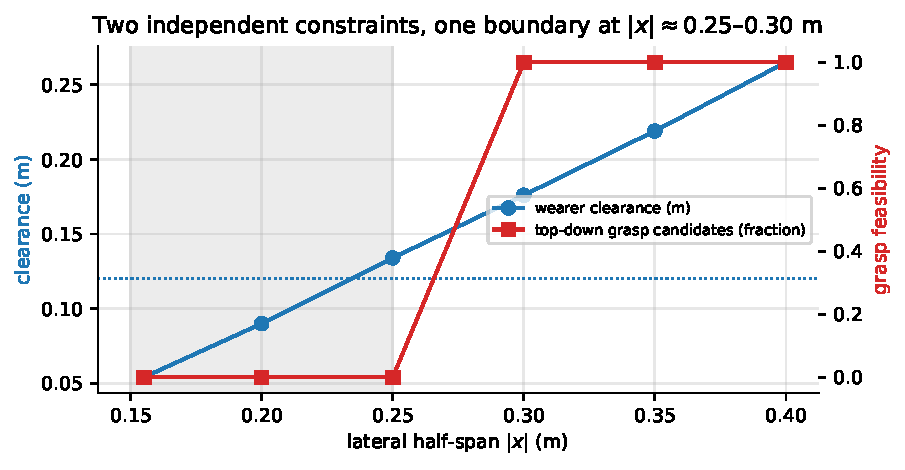
\includegraphics[width=0.85\textwidth]{figures/lateral_constraint.pdf}
  \caption[Two constraints, one boundary]{Wearer clearance and top-down grasp
  feasibility against lateral half-span. The two constraints were measured
  independently and for different purposes, and both place the usable boundary
  at $|x| \approx \SIrange{0.25}{0.30}{\metre}$.}
  \label{fig:lateral}
\end{figure}

\section{Consequences for the task set}

Three consequences follow directly, and each is visible in the task
definitions of \cref{ch:results}.

\textbf{Inter-arm handover is impossible.} It requires both arms at one point,
and no such point exists. This removes an entire task family, and no control,
planning or autonomy change can restore it.

\textbf{A bimanual task must either span the gap or exploit simultaneity.} A
rigid object held at two points can bridge the dead band; two targets in the
two disjoint sets can require simultaneous satisfaction. Both routes are used.

\textbf{The coupled objects had to be re-specified.} The original
\SI{310}{\milli\metre} tray placed each grip at $|x| = \SI{0.155}{\metre}$,
inside the dead band, and ten of twenty-five waypoints failed once the arms
were verified at home. Widening to \SI{500}{\milli\metre} places each grip at
$|x| = \SI{0.25}{\metre}$, which satisfies the clearance boundary and the
reachability boundary simultaneously. The compliant carrier had to lengthen
with it: retention of a ball of radius $r$ requires sag of at least $2r$, so

\begin{equation}
  \mathrm{sag}(s) = \sqrt{\left(\tfrac{L}{2}\right)^{2}
                          - \left(\tfrac{s}{2}\right)^{2}},
  \qquad
  s_{\max} = 2\sqrt{\left(\tfrac{L}{2}\right)^{2} - (2r)^{2}},
  \label{eq:sling}
\end{equation}

where $s$ is the gripper separation, $L$ the carrier length and $r$ the ball
radius. For $L = \SI{540}{\milli\metre}$ and $r = \SI{20}{\milli\metre}$ this
gives $s_{\max} = \SI{534}{\milli\metre}$, leaving a \SI{34}{\milli\metre}
margin at the nominal \SI{500}{\milli\metre} separation
(\cref{fig:sling}). The length is chosen so that the failure threshold sits
\emph{inside} the reachable band: a longer carrier could never fail and would
measure nothing.

\begin{figure}[htbp]
  \centering
  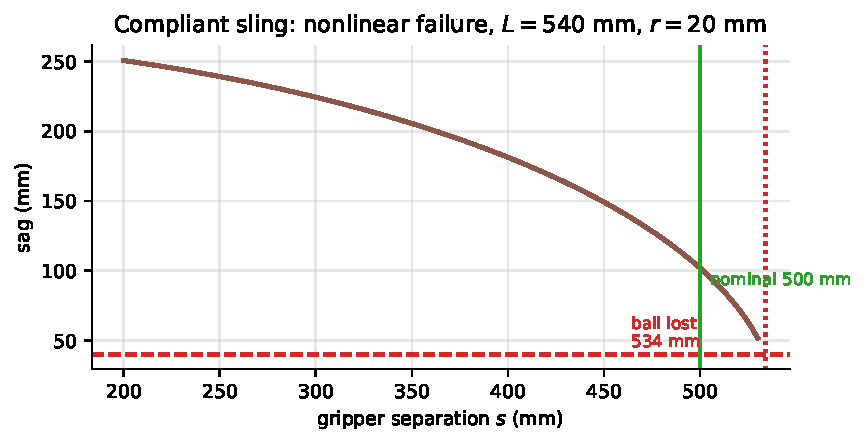
\includegraphics[width=0.8\textwidth]{figures/sling_geometry.pdf}
  \caption[Compliant carrier geometry]{Sag against gripper separation for the
  re-specified compliant carrier. The nonlinearity is the point: sag falls
  slowly, then the ball is lost abruptly at \SI{534}{\milli\metre}.}
  \label{fig:sling}
\end{figure}
